
\documentclass[12pt, oneside]{amsart}
\usepackage[font={sf}]{caption}
\usepackage[]{graphics}
\usepackage{graphicx}
\usepackage{epstopdf}
\usepackage{hyperref}
\hypersetup{breaklinks=true, colorlinks=true, citecolor=blue}
\usepackage{natbib}
\usepackage{color}
\usepackage{soul}
\usepackage{rotating}
\usepackage{tabularx}
\usepackage{longtable}
\usepackage{lscape}
\usepackage{array}
\usepackage{multirow}
\usepackage{setspace}
\usepackage{textcomp}
\usepackage{dcolumn}
\setlength{\LTcapwidth}{6in}
\usepackage{dcolumn}
\usepackage[margin=1in]{geometry}

 \bibpunct{(}{)}{,}{a}{}{,}
 \doublespacing
 \raggedright
 \setlength{\parindent}{15pt} 


\begin{document}
%\setcounter{secnumdepth}{0}


{ \Large \bf Figures}


%\tableofcontents
%\listoftables
%\renewcommand\thesection{S1}
%\listoffigures

\begin{figure}[h]
\begin{center}
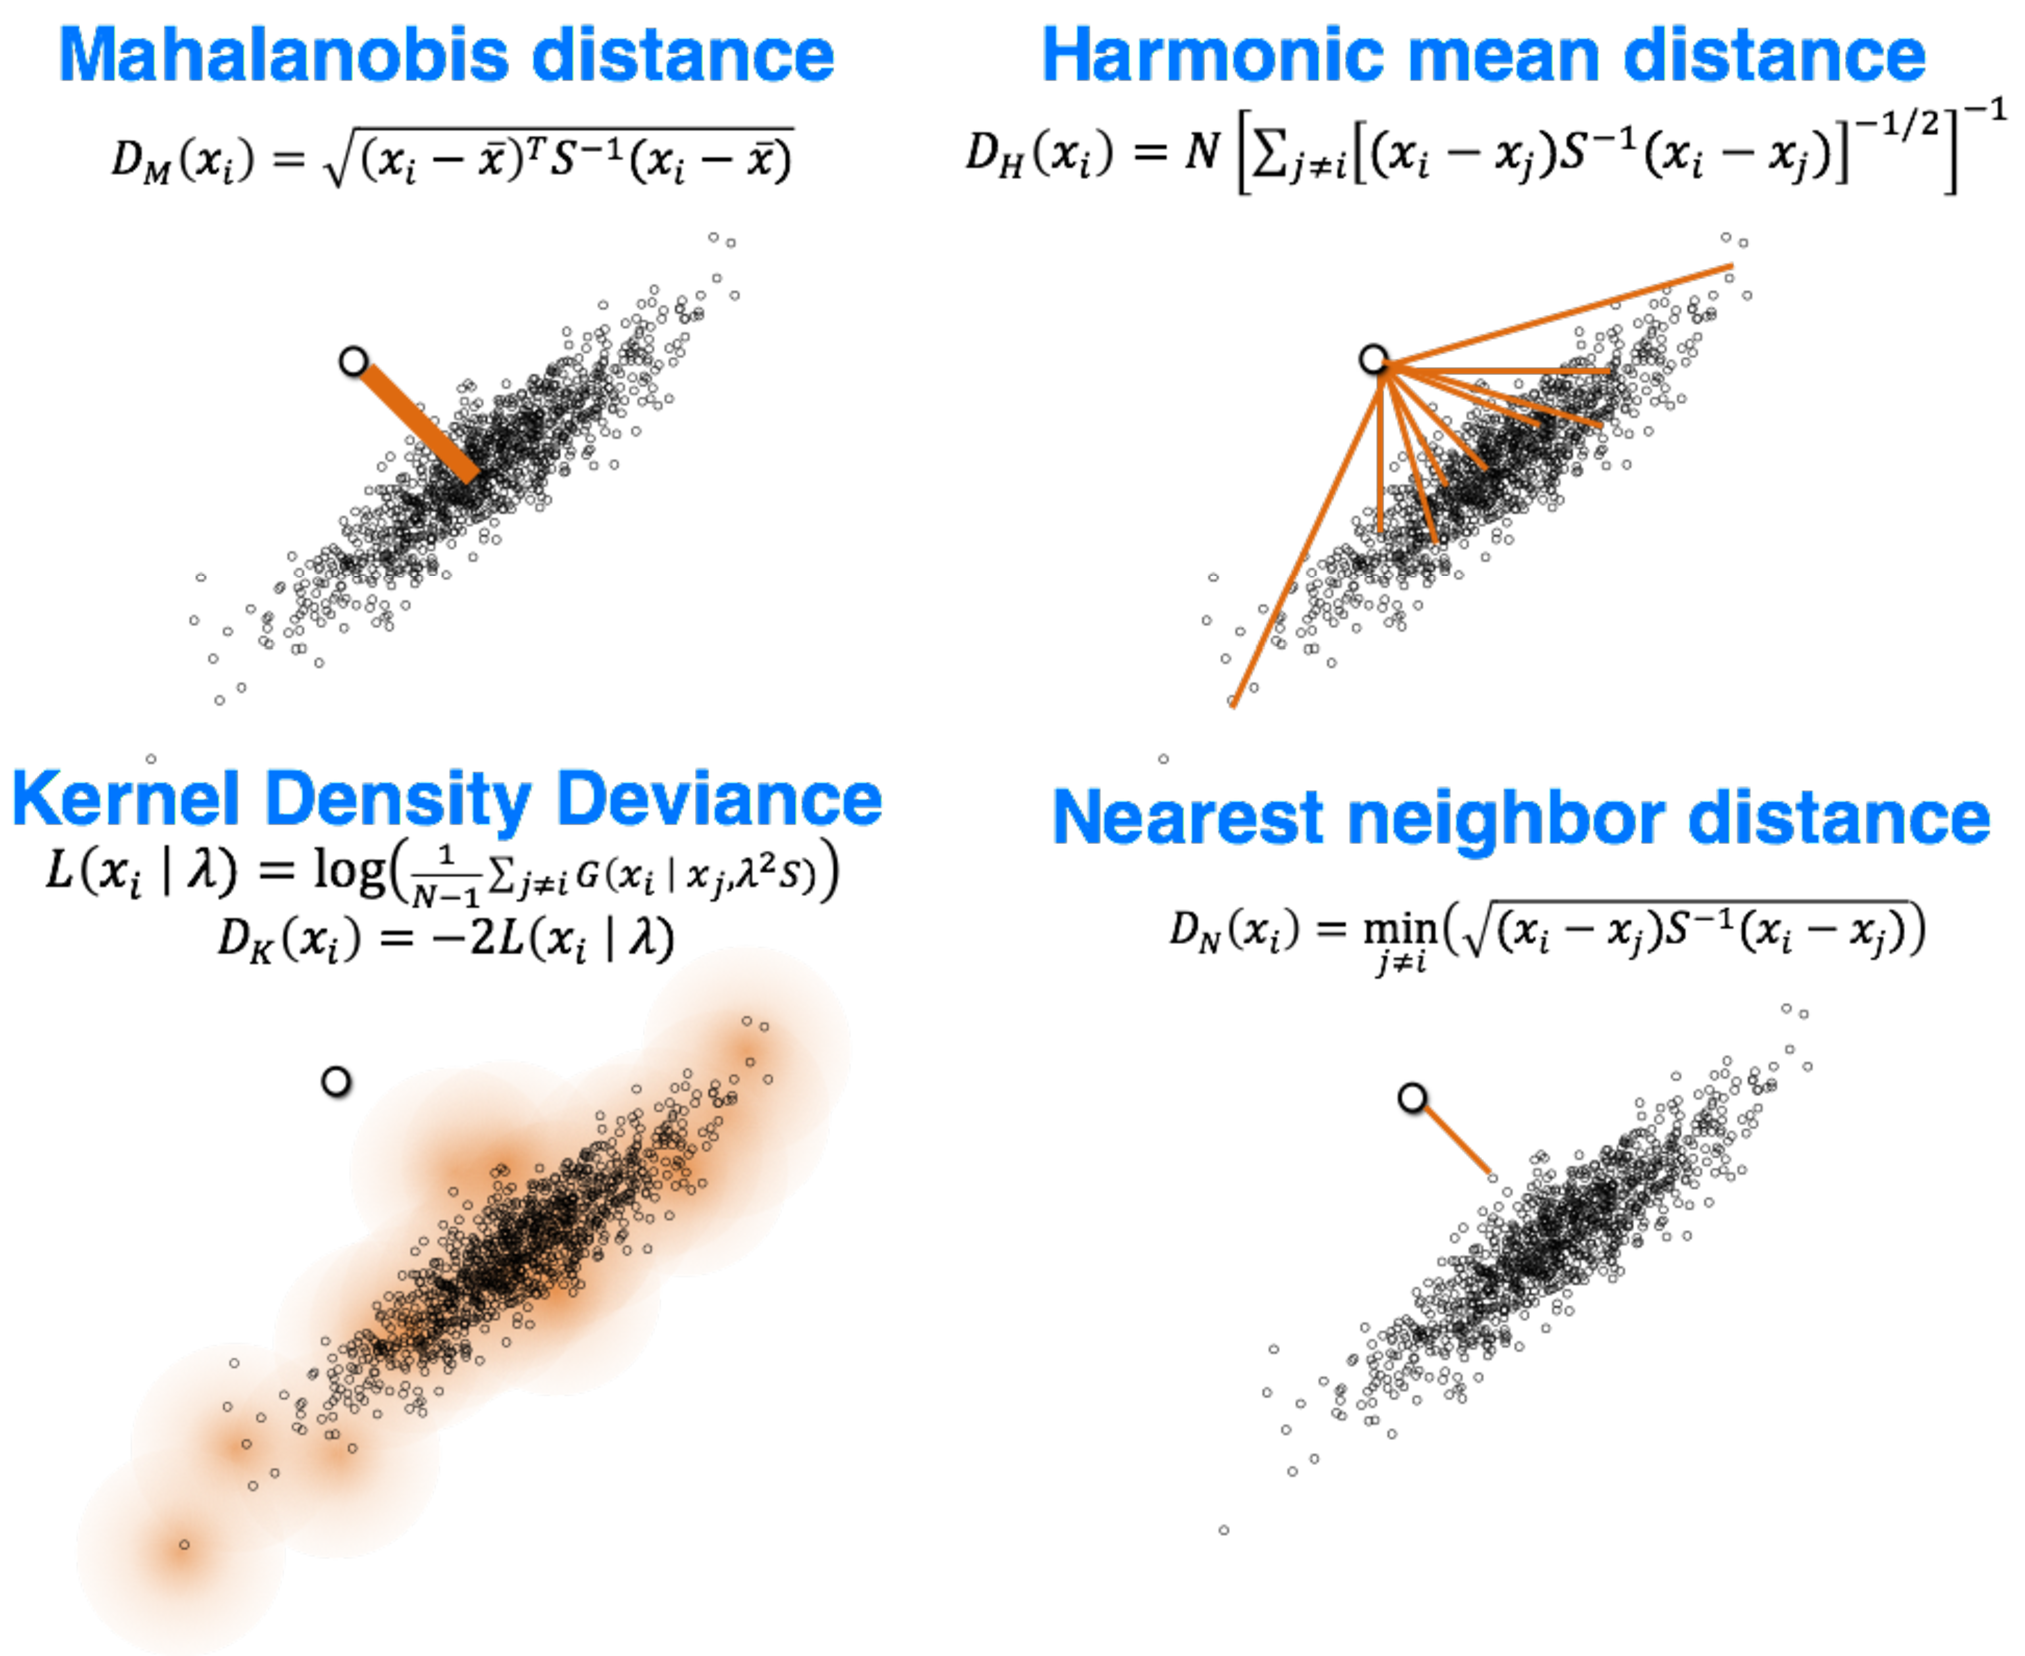
\includegraphics[width=6in]{../figures_man2/F1-FourMeasures.pdf}
\end{center}
\caption[]{Conceptual examples of the four multivariate statistics compared in this study. 

{\bf TO DO: Add ABCD.

TEAM: Would anyone like to take on making a figure like this one, but better for publication? I made these in power point, which is why they are awful. I think the kernel deviance could be challenging to visualize, because technically the bandwidth should be proportional to the variance in each dimension. The harmonic mean could also be challenging, because that is a lot of overlapping lines to draw. It might be good to draw the lines first with transparency=0.1 and lay the points on top.}} 
 \label{fig:???}
\end{figure}

\newpage
\begin{figure}[h]
\begin{center}
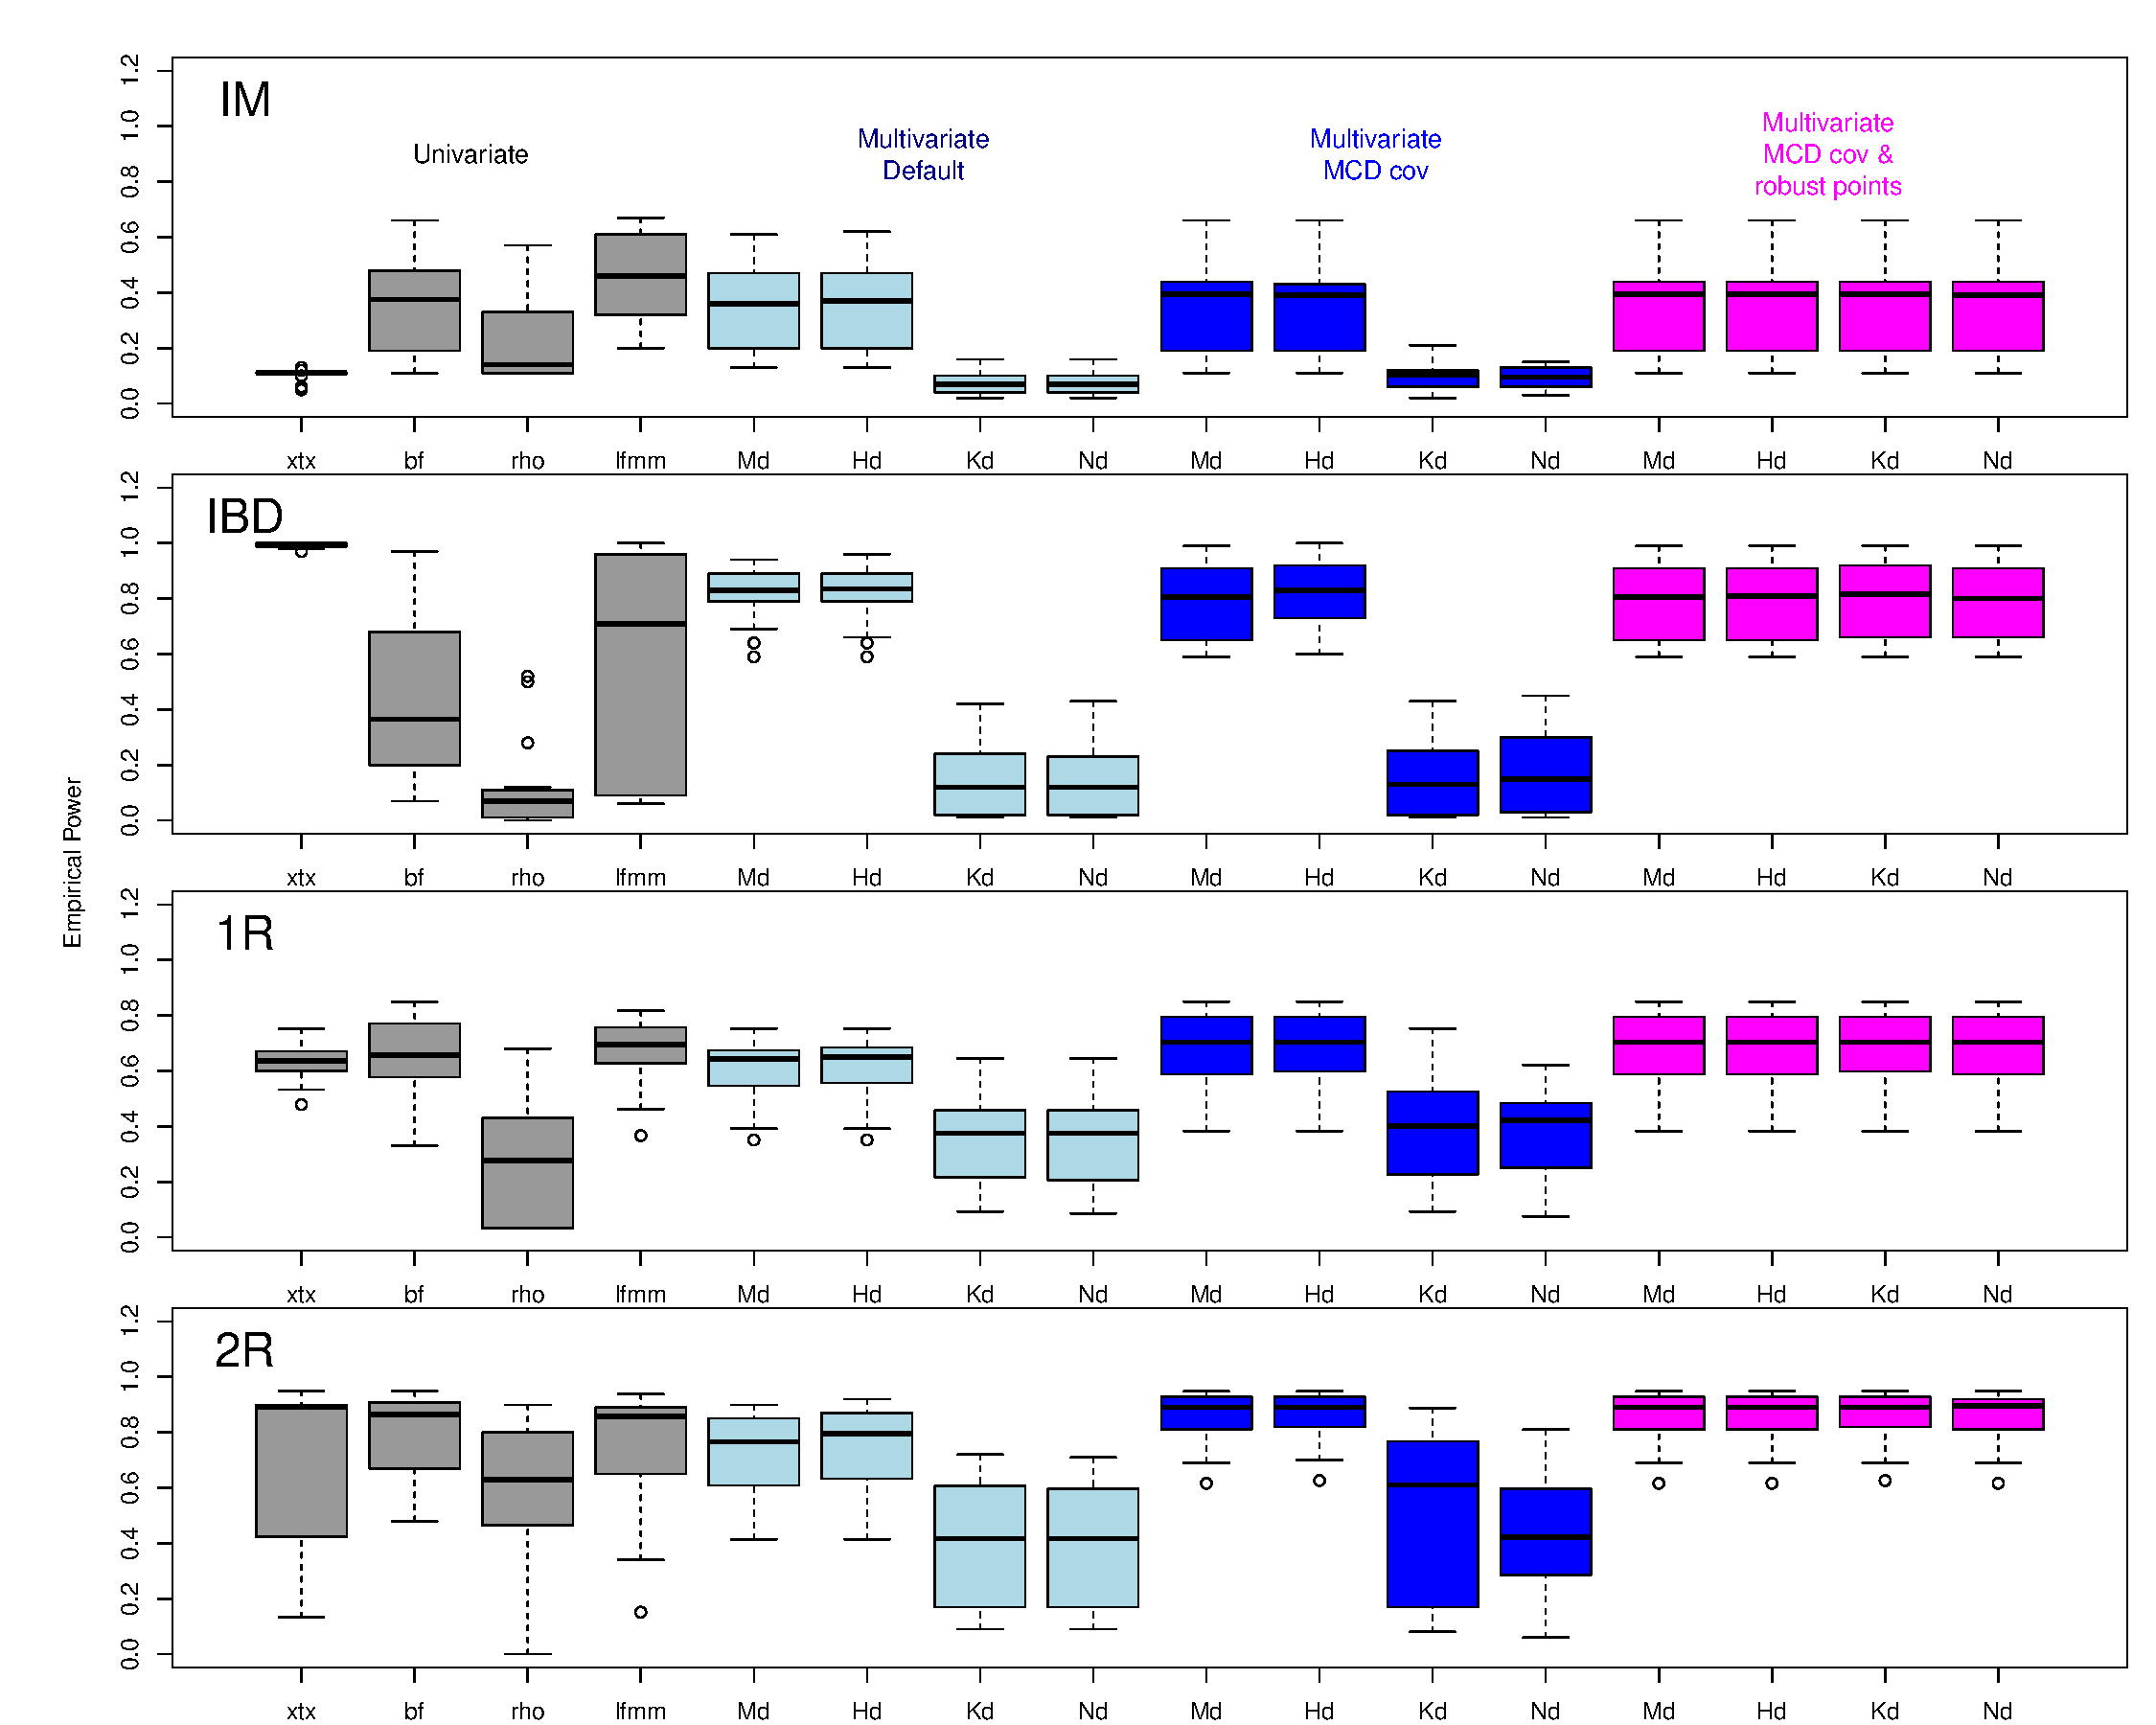
\includegraphics[width=6in]{../figures_man2/F2-LandsharcSummary.pdf}
\end{center}
\caption[]{Comparison of univariate and multivariate statistics for their power to separate signals of selection from neutrality. Each row represents one of the simulated demographies (IM = Island Model, IBD = Isolation By Distance, 1R = range expansion from one refuge, 2R = range expansion from two refugia). The four univariate statistics (grey box plots) evaluated were: $X^TX$ (xtx), Bayes Factors (bf), Spearman's $\rho$, and  $Z$-scores (lfmm).} 
 \label{fig:???}
\end{figure}


\newpage
\begin{figure}[h]
\begin{center}
\includegraphics[width=6in]{../figures_man2/F3-CovEllipse_4NeutralMCDpoints.png}
\end{center}
\caption[]{Comparison of 99\% confidence intervals on the two dimensional ellipse given by the determinant on the covariance matrix between these two variables calculated from: (i) all the data, (ii) neutral loci only, and (iii) the MCD estimate. 

{\bf TEAM: does this visualize that the robust points are neutral or is it unclear?

TO DO: Need to add legend to this plot (neutral = grey, triangles = different strengths of selection, pink dots = robust points).  Replace "xtx" with $X^TX$ and rho with Spearman's $\rho$. Maybe change the colors so that neutral ellipse is black, and change the lines so that it works in BW.
}
}
 \label{fig:???}
\end{figure}



\newpage
\begin{figure}[h]
\begin{center}
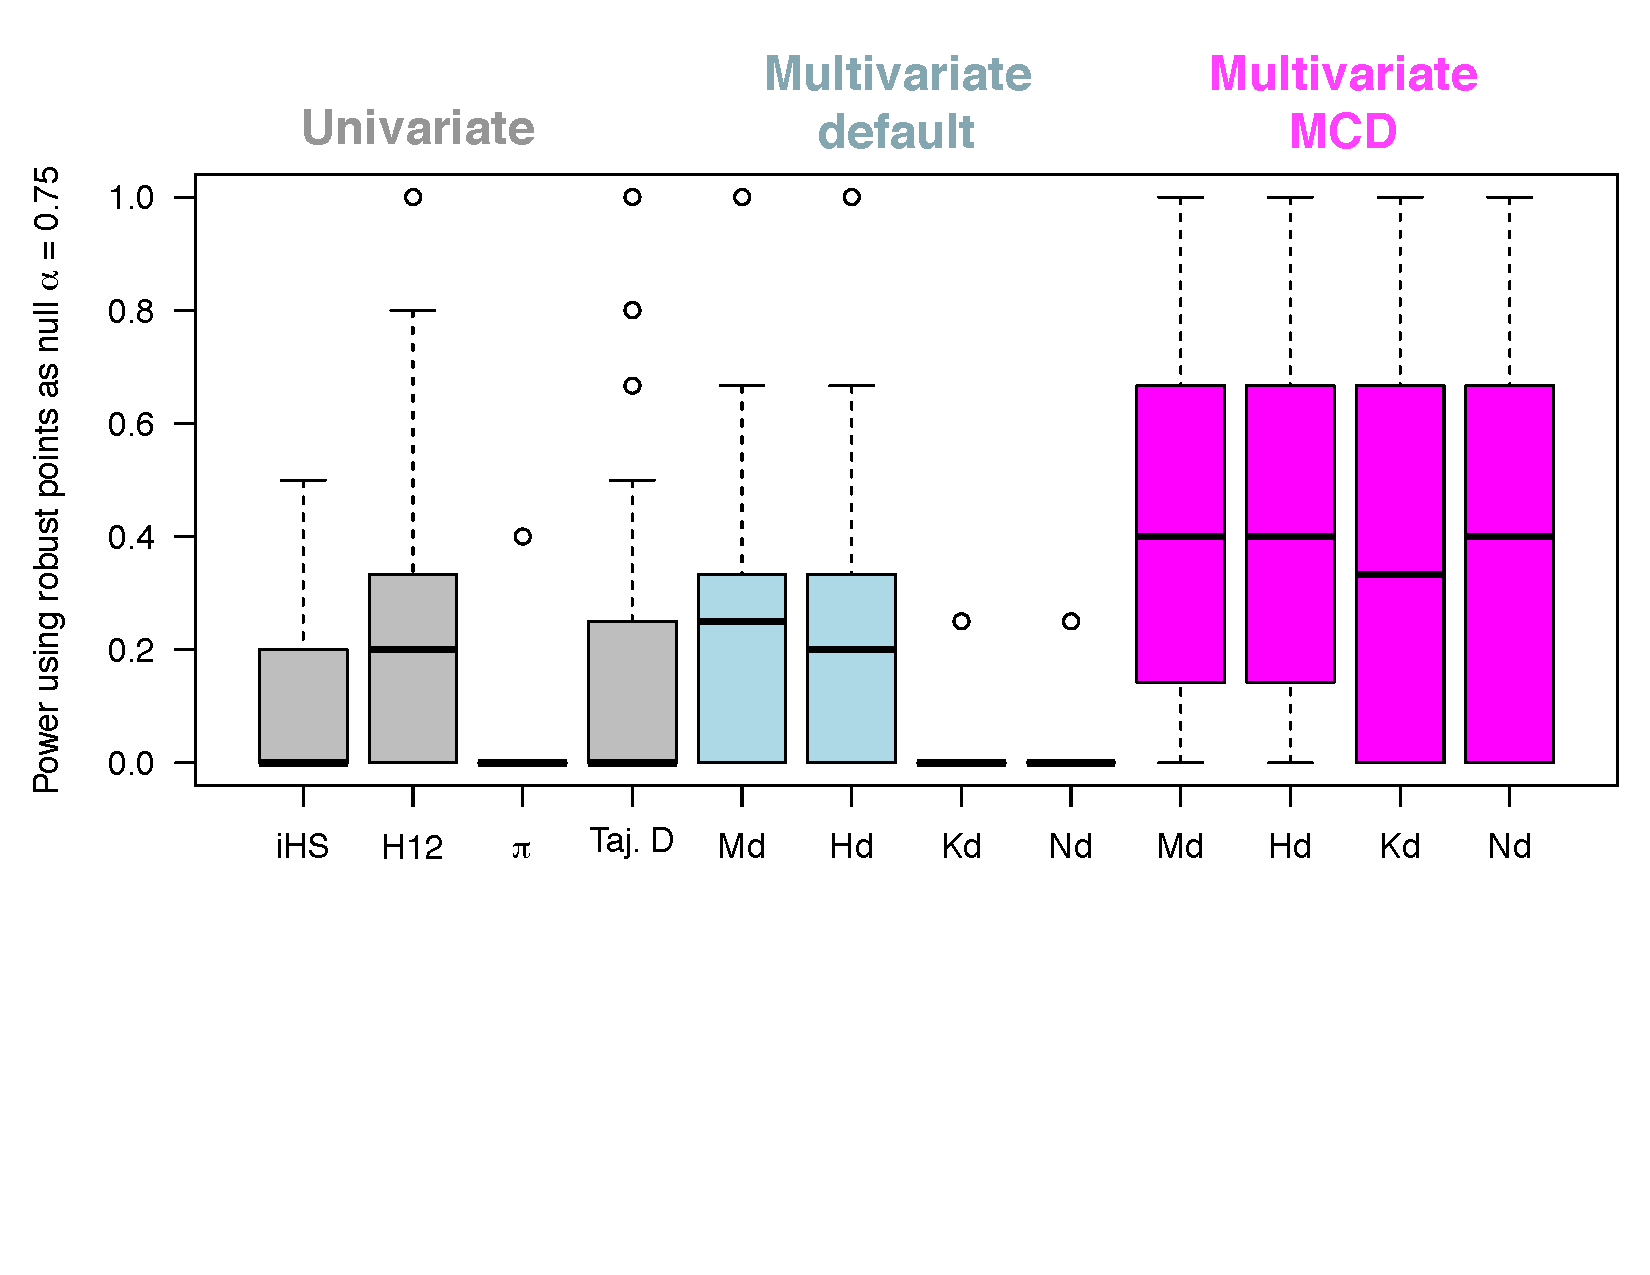
\includegraphics[width=4in]{../figures_man2/F4-DogPower_alpha075_title.pdf}
\end{center}
\caption[]{Comparison of power of different univariate and multivariate statistics to detect known QTL in the dog dataset. Power was evaluated as the proportion of known QTL with a signal above the maximum value of that statistic at the robust points identified by the MCD with $\alpha=0.75$. Multivariate "default" was calculated using all the data, while "MCD" was calculated using the MCD estimates of multivariate mean and covariance as well as the robust points in the calculation, if applicable.  Statistics evaluated include integrated haplotype score (iHS), H12, Tajima's D (Taj. D), nucleotide diversity ($\pi$), Mahalanobis distance (Md), harmonic mean distance (Hd), kernel deviance (Kd), and nearest neighbor distance (Nd). } 
 \label{fig:???}
\end{figure}


\newpage
\begin{figure}[h]
\begin{center}
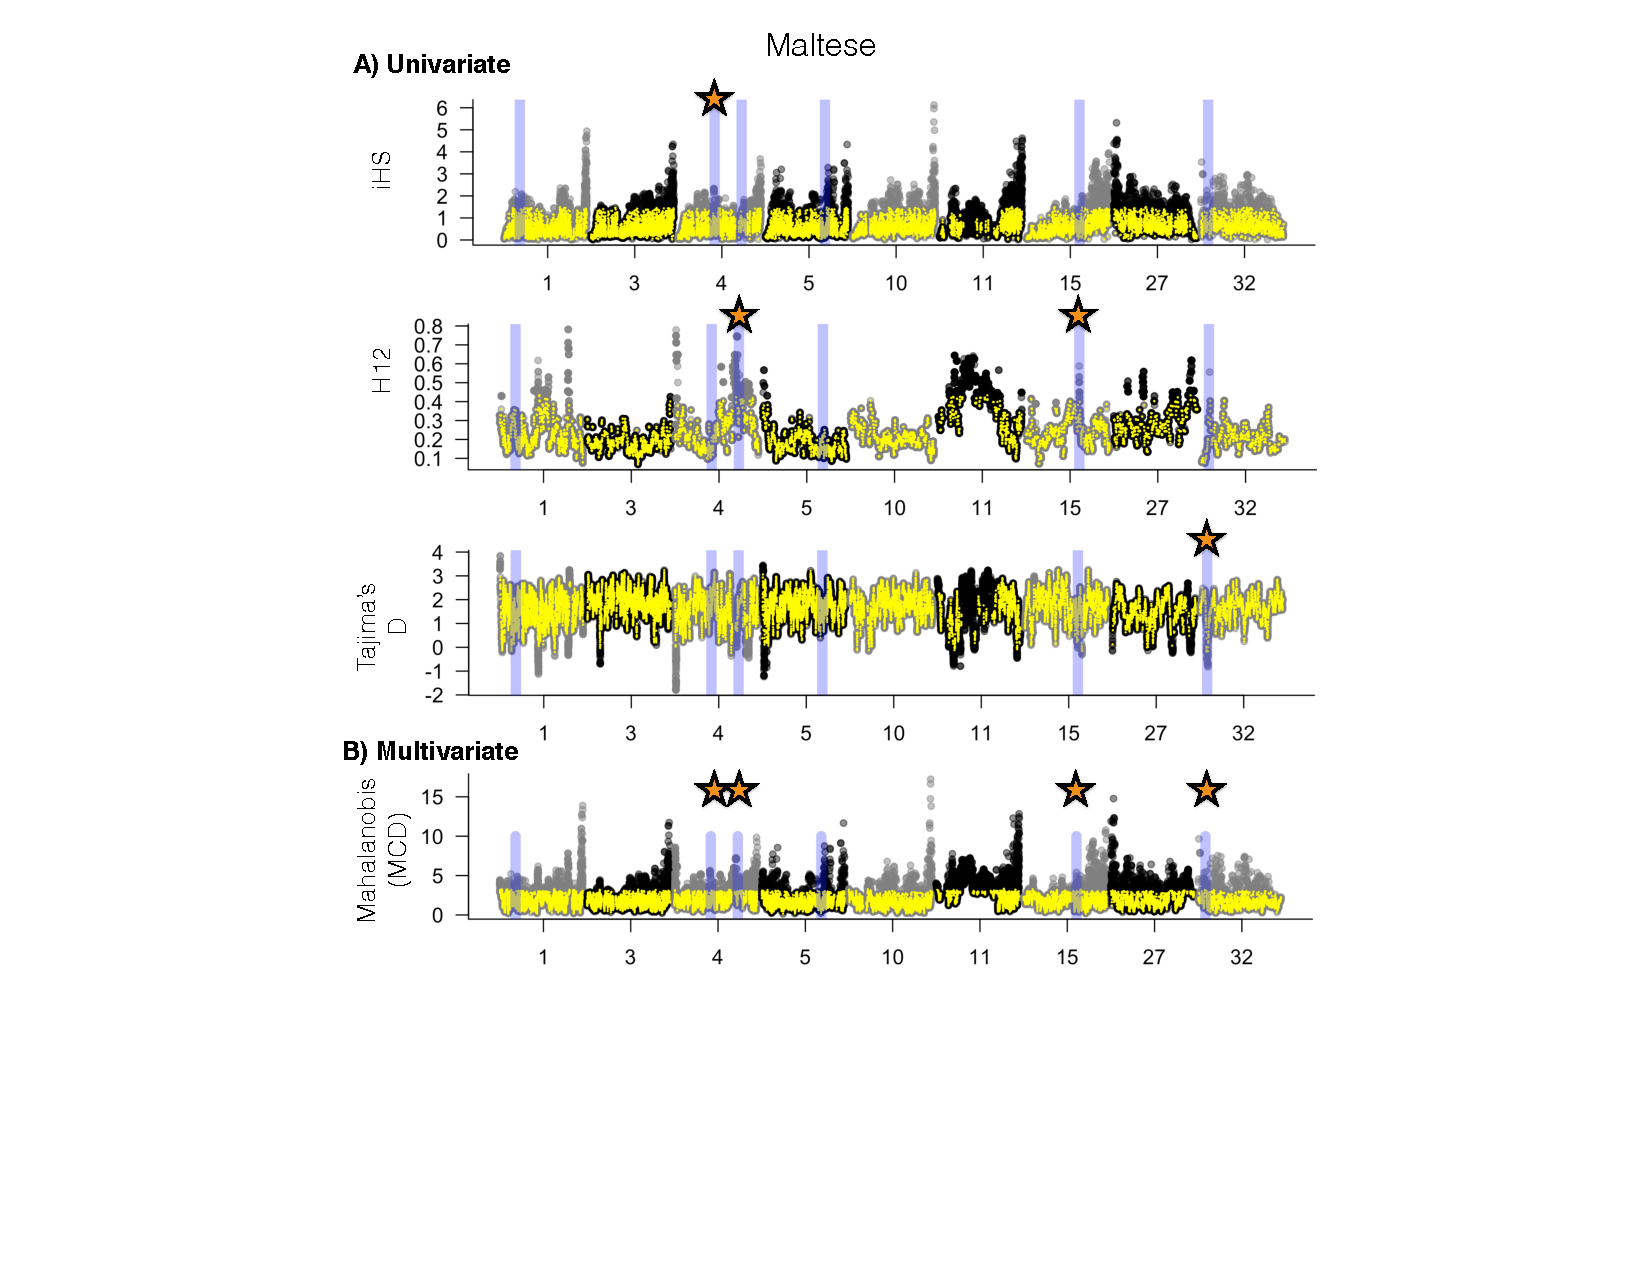
\includegraphics[width=4in]{../figures_man2/F5-MalteseManhattan.pdf}
\end{center}
\caption[]{Comparison of Manhattan plots for three univariate statistics (A) and the multivariate summary statistic of Mahalanobis distance (B). The points identified as robust in the MCD algorithm are highlighted in yellow. The vertical blue lines indicate the causal QTL that have risen to a frequency greater than 50\% in this breed, and the stars indicate whether that QTL is significantly greater than the threshold as described in the main text. The univariate statistics included in the multivariate calculation included integrated haplotype score (iHS), H12, Tajima's D, and nucleotide diversity ($\pi$, which is not plotted because it had no power to detect these QTL).} 
 \label{fig:???}
\end{figure}


\end{document}